
\chapter{Introduction}
\label{ch:Introduction}

\section{Context}
Parkinson’s disease is a chronic and progressive movement disorder caused by the malfunction and death of neurons in the brain. Some of these neurons produce dopamine, a chemical that sends messages to the part of the brain that controls movement and coordination. Thus, as Parkinson’s disease progresses,  the amount of dopamine produced in the brain decreases, leaving the person unable to control movement normally \cite{pdf}.

The disease must be diagnosed by an experienced neurologist. There are no tests that clearly identify the disease, but brain scans and blood test are sometimes used to rule out disorders that could give similar symptoms. 
One of the main concerns of people with PD is the fear of falling. First motor symptoms in this disease, like rigidity (stiffness  of the limbs and trunk), bradykinesia (slowness of movement) and postural changes, contribute to  risk of falling. Difficulties in the adaptation of neck and trunk cause  postural instability, which, in turn, increase the possibility of suffering a fall.

The center of body mass of a person is situated below the navel and the legs and works as a support base. In PD it is common that the center of  mass goes out of the support base. This fact causes losses of equilibrium in activities such as getting up, bending, spinning  around quickly or walking. Also, falls can occur due to a damage in postural reflexes (a series of complex movements that we carry out in an automatic way in order to maintain the equilibrium when we get up and walk), postural changes (tendency to lean forward using short, quick steps and reduced arm movement) and freezing (inability to step that delays gait initiation or interrupts ongoing gait). Research in this field is of vital importance to contribute to the improvement of advancement of knowledge about the disease. Scientific research can be the base for  field applications that help to improve the people life with PD\cite{ParkinsonDisease}\cite{pdf}. 

With this Project, we aim  to continue the research line initiated by Dr. Alberto Olivares, member of the SIPBA (Signal Processing and Biomedical Applications) research group of the Department of Signal Theory, Telematics and Communications of the University of Granada, Spain, and Prof. Dr. Med. Kai Bötzel, head of the Motion Analysis and Deep Brain Stimulation Laboratory of the Department of Neurology of the Klinikum Grosshadern based in Munich, Germany. In his Ph.D. dissertation, Dr. Olivares explains \cite{A.Olivares2013} different signal processing techniques to analyze information from inertial sensors to monitor human body motion.
Specifically, our work will be focused on signal processing of data gathered  by a force plate and a wearable motion analysis system based on inertial sensors, feature extraction and classification. Nevertheless, this master thesis is part of a broader project which has many different layers (instrumentation, data gathering, firmware, signal processing) in which other people have been working during the last 5 years.

 \begin{figure}[H]
 	\centering
 	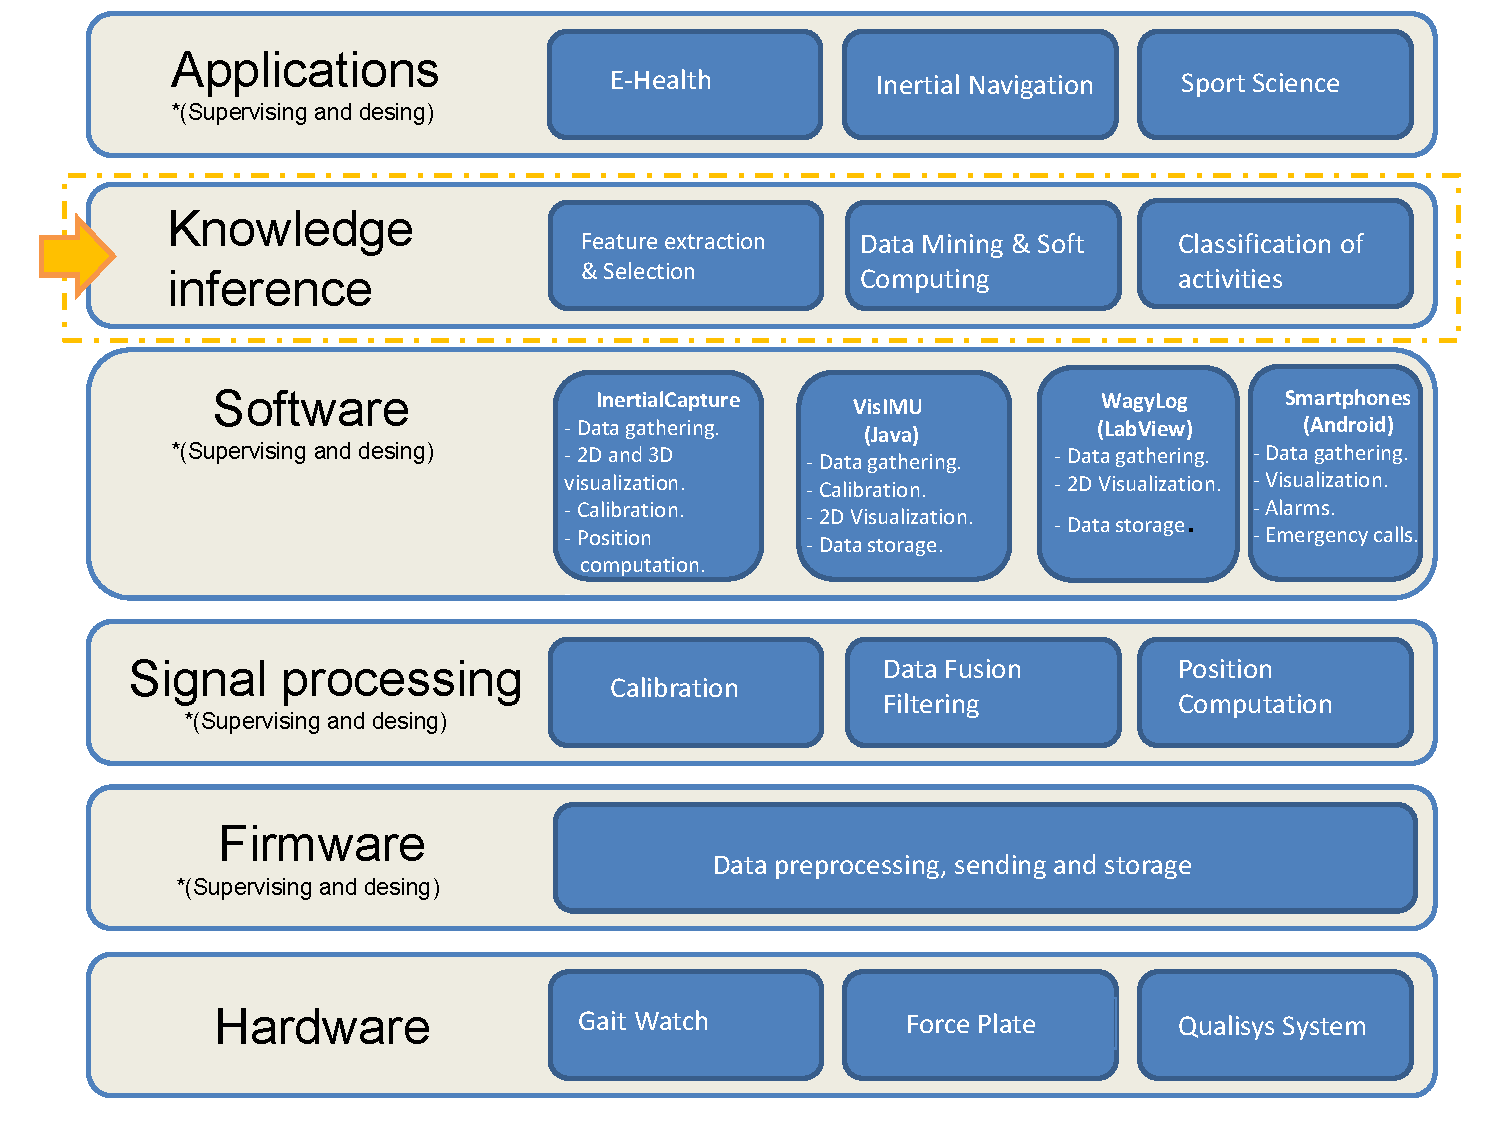
\epsfig{file=imagenes/Layer.pdf, width=17cm}
 	\caption{Layer structure of this project. Knowledge inference is highlighted as it includes the core of our work.}
 	\label{fig:layer}
 \end{figure}
 \vfill

\section{Motivation}
Parkinson’s disease is the second most common neurodegenerative disorder, it is extended globally and affects as much to men as to women. PD is more common among the population over 60 years old. It is estimated that seven  to ten million people worldwide are living with Parkinson’s disease. To this date, there is no cure to PD, so all efforts are focused on improving or prolonging the functionality of the patient for as long as possible. Therefore, it is an incentive to work in this field\cite{ParkinsonDisease}\cite{pdf}. 

Furthermore, Intel and Michael J.Fox Foundation have recently teamed up to create a sensor technology and analytics platforms for Parkinson’s treatment and monitoring. Fox Foundation CEO Todd Sherer told Fast Company \textit{'Parkinson’s is a motor disorder for the most part, with slowness of movement, tremors, falls, problems sleeping, and many disease symptoms. The way it is measured right now requires episodic periodic visits to a neurologist, who puts patients through fairly subjective and coarse clinical tests, there are many 1-2-3-4 scales. What we need to advance is research that is a much more consistent and objective measure of the disease. People live with Parkinson’s 24 hours a day, 7 days a week, not just when they're in the doctor’s office'}\cite{IntelAndMjf}.

The goal is to track the symptoms and progress of Parkinson’s disease day by day, and using this information to research the disease in depth.

\begin{figure}[H]
	\centering
	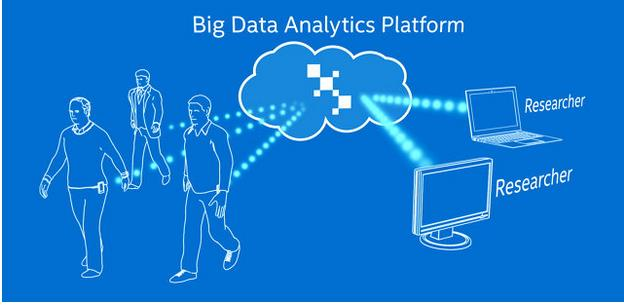
\epsfig{file=imagenes/IntelAndMjf, width=7cm}
	\caption{Illustration of sensors distribution thought up by Intel and Mjf\cite{IntelAndMjf}.}
	\label{fig:IntelAndMjf}
\end{figure}

Diane Bryant, senior vice president of Intel's Data Center Group, said in a release \cite{IntelAndMjf}
\textit{'Emerging technologies can not only create a new paradigm for measurement of Parkinson's, but as more data is made available to the medical community, it may also point to currently unidentified features of the disease that could lead to new areas of research'.}

\section{Goals}

The main goal of this project is to perform a thorough analysis of Anticipatory Postural Adjustments (referred to as APA in the remainder of this document) of PD patients. APAs can be used to characterize step initiation deficits in subjects with PD and also as a differentiating factor which may help early diagnosis of the disease.

To this purpose, we will make use of a database gathered by the medical team in Munich. The database contains both data from a force plate and inertial sensors. The patients wear the motion monitoring system containing the inertial sensors while they step on and down the force plate.

Once the measurements are made, the main objective is to determine whether it is possible to use inertial sensors to extract the information provided by the force plate. That is, we will evaluate the correlation between inertial sensor measurements and the force plate measurements in order to study the feasibility of the wearable device to study APAs in an ambulatory way. 

Furthermore, we will conclude determining whether it is possible to classify data force between Parkinson patients and control subjects for the diagnostic of this disease.

Additionally, we will try making a comparative study between the pitch angles calculated in both inertial sensors and Qualisys optical motion tracking system. The precision of this system allows its use as a reference system to evaluate portable
motion tracking systems such as the GaitWatch. To carry out this comparison, healthy people walked over a treadmill at different velocities.

In a nutshell, the ultimate goal is to determine whether doctors can substitute force plates (which strongly limit the range of action of the patients) by the inertial wearable system (which allows ambulatory analysis).


\section{Project structure}
This document presents a slight variation from the standard structure in which there is a chapter including all the theoretical basis, followed by another chapter including all the experiments, results and their discussion and a final chapter drawing the conclusions. Instead, every separate chapter has its own introduction, theoretical fundamentals, experiments, results, discussion of results and some brief conclusions. This structure makes every chapter self-contained and, therefore, they can be read separately.
 
Therefore the document is divided as follows; chapter \ref{ch:Introduction} presents a brief introduction to the project. This includes  context, motivation, goals and the state of the art; chapter \ref{ch:Hardware} deals with Hardware description used for the development of the project. In this chapter it is explained the basis of Gait Watch, the Force platform and the Qualisys System.; chapter \ref{ch:GWandFP} includes the protocol followed by the patient to do the experiments while the data were being gathered by the GaitWatch System and the Force Plate. Then, we explain the procedure to carry out the synchronisation between the signals of both systems. After this, we extract the interesting features of these signals to characterise the Anticipatory Postural Adjustments in Pakinson patients. In this section, one of the most interesting method used is the PCA algorithm to extract the relevant information of the data. At the end of this chapter we explain the results and some conclusion obtained from them; chapter \ref{ch:forceData} includes a new experiment with force sensors underneath feet. The data gathered with them are processed for feature extraction with PCA and PLS algorithms. Also it is carried out a classification between Parkinson patients and control subjects; chapter \ref{ch:GWandQS} talks about the comparison between the Gait Watch and the Qualisys system. This chapter includes, the same as in the previous case, a brief introduction, theoretical fundamentals to calculate the pitch angle in the Qualisys system, the feature extraction and the explanation of the results; chapter \ref{ch:Applications} shows some interesting applications in the healthcare field  like diseases and daily activities. Also, we propose a business idea thought during the development of the project as well as a canvas model that summarises the business plan; finally, chapter \ref{ch:Conclusions} includes the general conclusions and summarizes the most relevant parts of everything that is presented in the rest of the chapters. We also discuss about future research lines and how we will orient forthcoming work.

\textit{You can see a visual summary of the project structure in the first appendix.}

\section{State of the art}

We will start by studying some of the current devices used for body motion monitoring as well as their benefits.

Later we will search the methods and experimental procedures used in several studies to analyse of Anticipatory Postural Adjustments in different cases, as well as their applications.

Finally, we will speak about the most common calibration techniques, signal processing and classification.


\subsection{Instrumentation}

There are several device types used to measure APAs. The most important are: electromyographs, force platforms, inertial sensors and devices based on cameras. 

Electromyography (EMG) is a technique that gives us information about the electrical activity produced by skeletal muscles (See figure \ref{fig:Captura}). The electromyograph can detect  the electrical activity due to a electrical potential difference generated by muscle cells. It is very useful to analyse posture and to locate injuries like muscle paralysis \cite{Marcio2010} \cite{Instr1}. 


So far, most of studies have included like measurement devices, among other things, a platform sensitive to force and pressure. However, the cost and complexity of APAs measurement with a traditional movement analysis, using force platform and EMG System limit their applications in the  clinical practice. Therefore, small inertial sensors are used recently because they are cheaper and more portable. But even so, we have used this platform, considering the possibility to solely use inertial sensors in the future \cite{Mancini2009} \cite{Vennila2011}.

Devices based in commonly used inertial sensors are IMU (inertial measurement unit). IMUs are a electronic device that measures and reports about speed, orientation and gravity force of equipment, using a combination of accelerometers and gyroscopes.
In addition, these sensors can be combined with magnetometers to form a MIMU. Some current MIMUs are: 3DN-GX4-45 \cite{Instr2},  xsens-mvn \cite{Instr3} and mvn-biomech \cite{Instr4}, all of them use Microelectromechanical Systems (MEMS).

\begin{figure}[H]
	\centering
	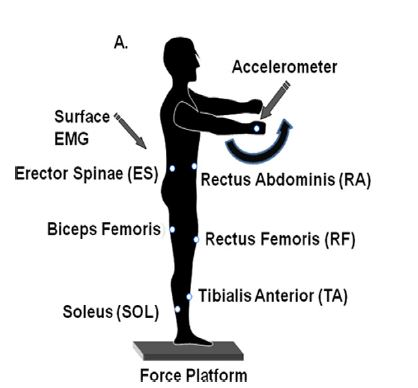
\epsfig{file=imagenes/Captura, width=7cm}
	\caption{EMG, accelerometers y platform \cite{Gay2011}.}
	\label{fig:Captura}
\end{figure}

There are  infrared-reflective markers that give us a complex posture measurement. They are attached  to the body and can provide information about postural strategies, so we can know if the subject uses the ankle strategy or the hip strategy. For example, figure \ref{fig:Captura2} shows the System.

\begin{figure}[H]
	\centering
	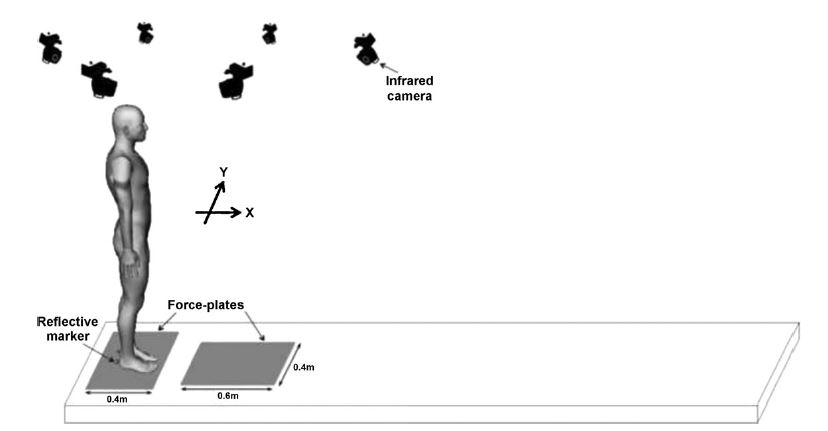
\epsfig{file=imagenes/Captura2, width=7cm}
	\caption{Illustration of the experiment with infrared-reflective markers\cite{Teddy2013}.}
	\label{fig:Captura2}
\end{figure}

As mentioned previously, it is possible to use sensors based on cameras that generally are part of an optical System of movement capture such as Kinect. \cite{Instr5}.


\subsection{Methods and procedure}

So far, a lot of studies about Anticipatory Postural Adjustments are been done, mainly in the last six years. The finality of most of this research is to be able to deepen knowledge about the posture prior to step initiation, and whether there are postural patterns and conditions on which they depend.

If we analyse the state of the art of APAs, we can find that first investigations tried to verify whether APAs are associated to conscious movements or not,  this hypothesis was confirmed and the conclusion was that it is more probable that the adjustments do not appear if step initiation is not planned. It is essential for balance control in gait initiation because we can use this knowledge to prevent the falls in some people with movement difficulties\cite{Mcllroy1993}\cite{Yiou2012}\cite{Teddy2013}\cite{Bouisset2008}\cite{Neeta2014}.

After this, researchers tried to explain the influence of other variables, such as several exercises that stimulate different muscles and the reaction of others\cite{Gay2011}; the age influence for generating postural patterns \cite{Bleuse2006} \cite{Estelle2008}; the signal type that initiates the movement ( visual or auditory) due that it affect initial posture \cite{Mcllroy1993}\cite{Antonia2009}\cite{Vicent1999}\cite{Tard2013}; the fear to fall because it can do that patients adopt different postures\cite{Chris2005}; neurodegenerative diseases like Parkinson and Multiple Sclerosis\cite{Mancini2009}\cite{Jebb2008}\cite{Chris2005}\cite{Hall2013}, or cerebral palsy, like hemiplegia and diplegia, \cite{Hall2013}, generate differences in the APAs too.

All these studies are very important in medical applications. For example, as mentioned previously, there are diseases that affect the Central Nervous System, so it affects the mobility too. Then, it causes falls in many occasions, therefore  people that suffer the fall have fear of falling again. The fact that fear of falling causes variations in the APAs making people fall again can help us to prevent this fact.

\subsection{Data Analysis}

In the last years, a lot of works about  calibration of accelerometers and gyroscopes have been carried out, although most of them show little variation with others studies done before. One of the most important research works  \cite{Kian2011} explains one form to do the calibration putting the accelerometers in six different positions and applying simple algebraic algorithms to the obtained data. The gyroscope is calibrated in a different way, using a process based in a known rotation. 

There are other methods that try to be more precise, increasing the number of positions where data are recorded \cite{Camps2009}. Also, there are others type of calibration techniques like algorithms based in basic algebraic calculation or in FIR filters \cite{A.Olivares2013}.

As for estimation of orientation for human-body monitoring, if we study the works done so far, we can see that almost all  use a Kalman Filter. However, the accuracy of Kalman filters can be poor if motion being monitored is intense \cite{A.Olivares2013}.

Finally, we will analyse the state of the art of movement recognition in humans, feature extraction and classifiers. Quickly, we can see a lot of information about classification because there are a lot of articles and books about this. However, there are others type of studies, that we will consider \cite{FrenkelToledo} \cite{Jeon}\cite{Banos2012}, that explain methods for obtaining gait features, pattern definition and human activity recognition based on a sensor weighting hierarchical classifier and others algorithms such as PCA and PLS \cite{Gorriz} \cite{pls_pca}. 
